\documentclass[10pt]{article}

\usepackage{fancyhdr}
\usepackage[includeheadfoot,left=1in, right=1in, top=0.5in, bottom=0.5in]{geometry}
\usepackage{lastpage}
\usepackage{extramarks}
\usepackage[usenames,dvipsnames]{color}
\usepackage{graphicx}
\usepackage{graphics}
\usepackage{listings}
\usepackage{courier}
\usepackage{float}
\usepackage{url}
\usepackage{subfigure}
\usepackage{varwidth}
\usepackage{caption}
\usepackage{multirow}
\usepackage[pdfborder={0 0 0}]{hyperref}
\usepackage[compact,small]{titlesec}
\usepackage{microtype}
\usepackage{verbatim}
\usepackage{booktabs}
\usepackage{indentfirst}
\usepackage{pgffor}
\usepackage[table]{xcolor}

\usepackage{amsmath}
%\usepackage[fleqn]{amsmath}

\rowcolors{2}{gray!25}{white}

\parskip = 0.5\baselineskip
\setlength{\belowcaptionskip}{-\baselineskip}

\captionsetup{font=scriptsize}
\captionsetup{labelfont=bf}

\pagestyle{fancy}
\rhead{Stack Attack}
\lhead{Network Security}
\rfoot{Page\ \thepage\ of \protect\pageref{LastPage}}
\cfoot{}
\renewcommand\headrulewidth{0.4pt}
\renewcommand\footrulewidth{0.4pt}

% make verbatim text small
\makeatletter
\g@addto@macro\@verbatim\tiny
\makeatother

\setlength\parindent{0pt} % Removes all indentation from paragraphs

\definecolor{sh_comment}{rgb}{0.12, 0.38, 0.18 } %adjusted, in Eclipse: {0.25, 0.42, 0.30 } = #3F6A4D
\definecolor{sh_keyword}{rgb}{0.37, 0.08, 0.25}  % #5F1441
\definecolor{sh_string}{rgb}{0.06, 0.10, 0.98} % #101AF9

\lstset{
    language=python,
    xleftmargin=.25in,
    xrightmargin=.25in,
    numbers=left,
    numberstyle=\tiny,
    frame=tb,
    showstringspaces=false,
    captionpos=b,
    stringstyle=\color{sh_string},
    keywordstyle = \color{sh_keyword}\bfseries,
    commentstyle=\color{sh_comment}\itshape,
    %basicstyle=\footnotesize\sffamily,
    basicstyle=\scriptsize\sffamily,
    %numbersep=-5pt,
    belowskip=\baselineskip,
    aboveskip=\baselineskip
}

\let\oldtabular\tabular
\renewcommand{\tabular}{\footnotesize\oldtabular}

\newcommand{\placementimage}[2]{
    \begin{figure}[H]
        \centering
        \includegraphics[width=\linewidth, height=4in, keepaspectratio]{#1}
        \caption{#2}
    \end{figure}
}

\newcommand{\specialcell}[2][c]{\textbf{\begin{tabular}[#1]{@{}c@{}}#2\end{tabular}}}

\title{
    %Cover page with student’s name, title of the report, date submitted and the
    %statement “Submitted as the Capstone Project for the Master of Engineering
    %Degree”
    \vspace{2in}
    \textmd{\textbf{CS6053 - Network Security}}\\
    \vspace{4in}
}
\author{\textbf{Stack Attack}}

\begin{document}
\maketitle
\newpage
\parskip = 0.2\baselineskip
\newpage
\tableofcontents
%\newpage
\listoffigures
\listoftables
%\lstlistoflistings
\parskip = 0.5\baselineskip
\newpage

\section{Introduction}
The purpose of this lab was to create a program on the client end that connects
to a server. On the server end is another program that is running called the
\texttt{Monitor}. The \texttt{Monitor} listens for an open socket on an open
port for incoming connections. As long as the \texttt{Monitor} is able to
authenticate the client, the \texttt{Monitor} will reward points. The group with the
highest points wins the contest. The challenging part of the contest is to
remain a secure connection between the client and the server so the group is
able to be rewarded with points. In order to maintain a secure connection we
have implemented a few algorithms: Diffie-Hellman, Karn Symmetric Cyrptosystem,
and the Fiat-Shamir Algorithm.

\section{Implementation}

\subsection{Authentication of Monitor}
In order to authenticate with the \texttt{Monitor} we first needed to implement
a shared secret key. We did this by implementing the Diffie-Hellman protocol. The
Diffie-Hellman key exchange works as shown below:
\begin{figure}[H]
    \centering
    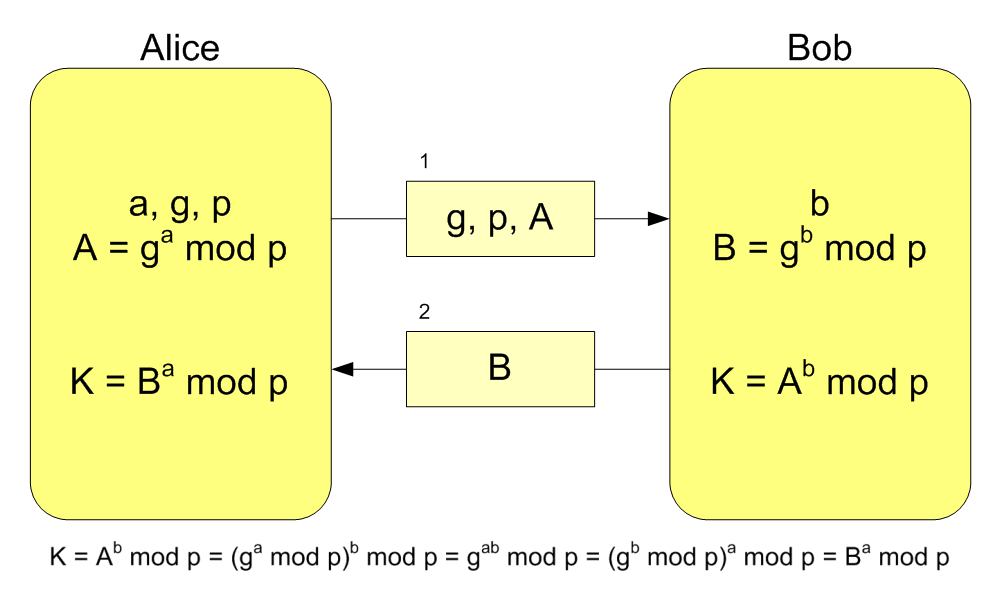
\includegraphics[width=\linewidth]{./pics/diffie_hellman.png}
    \caption{Diffie-Hellman Key Exchange}
\end{figure}
In the image above, we can see that the \texttt{g,p} are just the generator and
the modulo prime number respectively. \texttt{A} is calculated using the
function (g$^{a}$ mod p) sent over to \texttt{Bob}. Note that g,p, and A are all
seen by everyone. The trick here is that \texttt{Alice} and \texttt{Bob} both
generate there own secret key locally (this key is never sent). The way we can
authenticate can be shown in the example below:

\begin{align*}
    A &= g^{a} \thickspace mod \thickspace p,  \\
    B &= g^{b} \thickspace mod \thickspace p,  \\
    A &= 3^{15} \thickspace mod \thickspace 17 \equiv 6 \\
    B &= 3^{13} \thickspace mod \thickspace 17 \equiv 12 \\
    %t_{r} = R_{p}C ,
    %t_{f} = R_{n}C \\
    %R_{n} \propto {L_{n} \over W_{n}\mu_{0_{n}}},
    %R_{p} \propto {L_{p} \over W_{p}\mu_{0_{p}}}
\end{align*}
where a = 15 (Alice's secret key), g = 3, p = 17 and \\
where b = 13 (Bob's secret key),   g = 3, p = 17 \\

Therefore, \texttt{Bob} receives this value from \texttt{Alice} along with p
and g. Now \texttt{Bob} computes his result and sends \texttt{12} to Alice. Now
the heart of the trick lies here: Alice will take Bob's message and use her
private key to get the correct message from Bob:

\begin{align*}
    A &= 12^{15} \thickspace mod \thickspace 17 \equiv 10 \\
    B &= 6^{13} \thickspace  mod \thickspace 17 \equiv 10
\end{align*}

The reason this works is because when you take an exponent to another exponent, these values get
multiplied:

\begin{align*}
    3^{13^{15}} \thickspace mod \thickspace 17 \equiv 3^{15^{13}} \thickspace mod \thickspace 17
\end{align*}

Therefore, even if Eve performed a man-in-the-middle attack, all Eve would have
is just the encrypted message and the prime and the generator number--making it
rather difficult to decrypt the message via brute-forcing due to the discrete
logarithm problem.

% encrypting with symmetric key
\subsection{Karn Symmetric Cryptosystem}
After implementing the Diffie-Hellman protocol we then needed to implement the
Karn encryption scheme. The Karn encryption scheme uses the Secure Hash
Algorithm (SHA-1) in order to generate the message digests. This algorithm uses
the shared keys generated by the Diffie-Hellman protocol. It initially splits
the bits of the shared secret key into two halves: a left and a right half. The
encryption algorithm works as described below:
\begin{itemize}
    \item Add ``guard'' byte of value 42,
    \item During each clock of plaintext, divide block of plaintext into
          left/right half,
    \item Find the message digest of the concatenation of the left plaintext
          half and the left key half,
    \item XOR the digest with the right plaintext half. (This produces the
          right ciphertext half),
    \item Find the message digest of the ciphertext right half concatenated
          with the key right half,
    \item XOR the digest with the plaintext left half.
\end{itemize}
Once this is complete we have both halves, therefore we can just output both the
left and right half of the ciphertext.

In order to decrypt the message we needed to follow the steps shown below:
\begin{itemize}
    \item Strip guard byte,
    \item For each ciphertext block, split the block into a left half and a
          right half,
    \item Find the message digest of the ciphertext right half concatenated
          with the key right half,
    \item XOR the result with the ciphertext left half to obtain the plaintext
          left half,
    \item Find the message digest of the plaintext left half and the key left
          half,
    \item XOR the result with the ciphertext right half to get the plaintext
          right half.
\end{itemize}

\subsection{Zero-Knowledge Proof}

% creating session key
\subsection{Diffie-Hellman}

\subsection{Maintaining Security}

%\begin{figure}[H]
%    \centering
%    \includegraphics[width=\linewidth]{./pics/mitm_attack.jpg}
%    \caption{Man-In-The-Middle Attack}
%\end{figure}

\newpage
\section{Appendix}
    \subsection{Python Code}
    \lstinputlisting[caption=\textbf{Client}]{../client.py}
    \lstinputlisting[caption=\textbf{Server}]{../server.py}
    \lstinputlisting[caption=\textbf{Diffie Hellman}]{../diffie_hellman.py}
    \lstinputlisting[caption=\textbf{Karn}]{../karn.py}
    \lstinputlisting[caption=\textbf{Fiat-Shamir - Zero Knowledge Proof}]{../fiat.py}
    \lstinputlisting[caption=\textbf{Printer}]{../printer.py}
    \lstinputlisting[caption=\textbf{Base 32}]{../base32.py}
    \lstinputlisting[caption=\textbf{Configuration File}]{../config.py}
    \lstinputlisting[caption=\textbf{Test 1}]{../test.py}
    \lstinputlisting[caption=\textbf{Test 2}]{../test2.py}

\newpage
\begin{thebibliography}{9}
    \bibitem{ssl} \url{http://www.digicert.com/sha-2-ssl-certificates.htm}
\end{thebibliography}

\end{document}
